\documentclass[]{aa} %bibnumber

%\usepackage{hyperref}
\usepackage{txfonts}
\usepackage{amsmath}
\usepackage[colorlinks,breaklinks]{hyperref}
\hypersetup{linkcolor=blue,citecolor=blue,filecolor=black,urlcolor=blue}


\usepackage{color}
\newcommand{\mr}[1]{{\textcolor[rgb]{0.60,0.10,0.6}{#1}}}
\newcommand{\mri}[1]{{\textcolor{red}{#1}}}
\newcommand{\nn}[1]{{\textcolor[rgb]{1, 0.27, 0}{#1}}}

\def\l{\lambda}\def\L{\Lambda}

\newcommand{\prob}[2]{\mathcal{P}\left( #1 \mid #2\right)}

\begin{document}
\title{Redshift Evolution of the Type Ia Supernova Population Stretch
Distribution}

\author{N. Nicolas
\thanks{n.nicolas@ipnl.in2p3.fr, equal contribution}
\inst{1}
    \and M. Rigault
\thanks{m.rigault@ipnl.in2p3.fr, equal contribution}
\inst{2}
    \and R. Graziani\inst{2}
    \and M. Briday\inst{1}
    \and Y. Copin\inst{1}
    \and Y. Kim\inst{1}
}

\institute{Université de Lyon, F-69622, Lyon, France; Université de Lyon
    1, Villeurbanne; CNRS/IN2P3, Institut de Physique des Deux Infinis, Lyon
    \and Université Clermont Auvergne, CNRS/IN2P3, Laboratoire de
    Physique de Clermont, F-63000 Clermont-Ferrand, France.
}

\date{Received 2 November 1992 / Accepted 7 January 1993}

\abstract{\mr{ABSTRACT NOT DONE YET.}
Type Ia supernovae (SNe Ia) allow for the construction of the Hubble
    diagram, giving us information about the Universe's expansion and its
    fundamental components, one of which is dark energy. But systematic
    uncertainties are now starting to be limiting in our ability to measure
    those parameters. In particular, the physics of SNe Ia is still mostly
    unknown, and is thought not to change in time/with the redshift.}
    {In an attempt to reduce those uncertainties, we try to find an empirical
    law describing SNe Ia's length of explosion (stretch) evolution with the
redshift.}
    {We started by getting a complete sample representing all of the stretch
        distribution that Nature can give us, before using LsSFR measurements,
        an age tracer which evolution with redshift is known, that has been
        shown to have a strong correlation with the stretch. We compare their
        AIC, an estimator of the relative quality of statistical models that
    includes the number of free parameters, to determine which ones describe
best the data.}
    {Models with an evolution of the stretch with the redshift have a better
    AIC than the ones without.}
    {We find that implementing these models allows us to fit the data better
    than models without stretch evolution.}

\keywords{Cosmology -- Type Ia Supernova -- Systematic uncertainties}
\maketitle

\section{Introduction}
Type Ia supernovae (SNe Ia) are powerful cosmological distance indicators that
have enabled the discovery of the acceleration of the Universe's expansion
\citep{riess1998, perlmutter1999}. They remain today a key cosmological probe to
understand the properties of dark energy (DE) as it is the only tool able to
precisely map the recent expansion rate $z<0.5$, when DE is driving it
\citep[e.g.][]{scolnicastro2020}. They also are key to directly measure the
Hubble Constant (H$_0$), provided one can calibrate their absolute magnitude
\citep{riess2016, freedman2019}. Interestingly, the value of H$_0$ derived when
the SNe~Ia are anchored on Cepheids \citep[the SH0ES
project][]{riess2009,riess2016} is $\sim5\sigma$ higher than what is predicted
by cosmic microwave background (CMB) data measured by Planck assuming the
standard $\L$CDM\nn{,} or when the SN luminosity is anchored at intermediate
redshift by the baryon acoustic oscillation (BAO) scale
\citep{riess2019,reid2019,planck2016, feeney2019}.  While using the tip of the
red giant branch technique in place of the Cepheids seem to favor an
\mr{intermediate} value of H$_0$ \citep{freedman2019}, time delay measurements
from strong lensing seem to also favor high H$_0$ values \citep{wong2019}.

The H$_0$ tension has received a lot of attention as it could be a sign of new
fundamental physics. Yet, no simple solution is able to accommodate this H$_0$
tension when accounting for all other probes \citep{knox2019} and the current
most promising scenario appears to be a burst of expansion at the
matter-radiation decoupling moment caused by a (fine tuned) early dark energy
\citep{poulin2019}.

Alternatively, systematic effects affecting one or several of the aforementioned
analysis could also explain the tension.  In \cite{rigault2015} we suggested
that SNe Ia from the Cepheid calibrator sample differs by construction from  the
Hubble flow as it strongly favors young stellar population environments where
one could find Cepheids. This selection effect would impact the derivation of
H$_0$ if SNe~Ia from young and older environments differ in average magnitudes. 

For the last decades, numerous analysis have studied the relation between SNe~Ia
and host properties\nn{,} finding first that the standardized SNe~Ia magnitude
significantly depends on the host stellar-mass, SNe~Ia from high-mass host
\nn{being brighter on average}
\cite[e.g.][]{kelly2010,sullivan2010,childress2013,betoule2014,rigault2018}.
This mass-step correction is currently used in cosmological analyses
\citep[e.g.][]{betoule2014,scolnic2018a}, including for deriving H$_0$
\citep{riess2016,riess2019}. Yet, the underlying connection between the SN and
the host remains unclear when using global properties such as the host stellar
mass, which raises the question of the accuracy of the correction. More
recently, studies have used the local SN environment to probe more direct
connections between the SN and its environments \citep{rigault2013}\nn{,}
showing that local age-tracers such as the local specific star formation rate or
the local color are more strongly correlated with the standardized SN magnitude
\citep{rigault2018,roman2018}, suggesting the age to be the driving parameter
underlying the mass-step. If true, this would have a significant impact for
cosmology because the redshift drift magnitude correction to apply might
strongly vary \citep{rigault2013,childress2014,scolnic2018a}.  Yet, the
importance of local SN environmental study remains highly debated
\cite[e.g.][]{jones2015,jones2019} and especially the impact it has on the
derivation of H$_0$ \cite{jones2015,riess2016,riess2018,rose2019}. 

In this paper, we take a step aside to probe the validity of our modeling of the
SN population that we claim to be constituted of two age-populations
\citep{rigault2013,rigault2015,rigault2018}: one old and one young, the former
having on average lower lightcurve stretches and being brighter after
standardization. We indeed use the correlation between the SN age probed with
local specific star formation rate in \cite{rigault2018} and the SN stretch to
model the expected evolution of the underlying SN stretch distribution as a
function of redshift. This modeling relies on three assumptions: (1) there
\nn{are indeed} 2 populations of SNe~Ia; (2) the relative fraction of each of
these populations as a function of redshift follows the age-modeling made in
\citep{rigault2018} and (3) the underlying distribution of stretch for each
age-sample can be modeled and do not significantly drift. This paper aims at
testing this with data from the literature. 

% SERIES OF PAPER
%This paper is part of a series of papers where we test the validity of the two
%SNe Ia population models developed in \citep{rigault2018}. Briday et al. in
%prep will present how using different environmental tracer is affecting our
%ability to distinguish the two populations, and Rigault et al. in prep will
%further study the connection with H$_0$. Here we analyze predictions concerning
%the SNe Ia redshift drifts: (1) that the distribution of the SN~Ia stretch, a
%purely intrinsic SN~Ia property, is evolving as a function of redshift and (2)
%that this population-drift follows the relation that \citep{rigault2018}
%derived assuming that one population is “young“ with a rate proportional to the
%star formation rate in the Universe and the second is "old" with a rate
%proportional to the stellar mass.

The concept of the SNe~Ia age dichotomy arised when the SN~Ia rate has first
been studied. \cite{mannucci2005, scannapieco2005, sullivan2006, aubourg2008}
have shown that the relative SNe~Ia rate in galaxies could only be explained if
two populations existed, one young, following the host star formation activity,
and one old following the host stellar mass (the so called “prompt and delayed“
or “A+B“ model). In \cite{rigault2018} we used the specific star formation rate
at the SN location (Local sSFR or LsSFR) to classify which are the prompts
(those with a high LsSFR) and which are the delayed (those with low LsSFR).
Furthermore, since the first SNe~Ia host analysis, the SN stretch has been known
to be strongly correlated with the SN host properties \citep{hamuy1996,
hamuy2000}, which has been extensively confirmed since \citep[e.g.][]{neill2009,
sullivan2010, lampeitl2010, kelly2010, gupta2011, dandrea2011, childress2013,
rigault2013, pan2014}. Following the “A+B“ model and the connection between SN
stretch and host properties, \cite{howell2007} first discussed the potential
redshift drift of the SN stretch distribution. In this paper we revisit this
analysis with the most recent SNe~Ia dataset..

We present in section~\ref{sec:sample} the sample we are using for this
analysis, which is based on the Pantheon dataset \citep{scolnic2018a}. We
discuss the importance of obtaining a "complete" sample, i.e. representative of
the true underlying SNe Ia distribution, and how we build one from the Pantheon
sample.  We then present in section~\ref{sec:modeling} our modeling of the
distribution of stretch as a function of redshift based stretch distribution of
young and old SNe~Ia. Our results are presented in section~\ref{sec:results}
where we test if the SN stretch does evolve as a function of redshift and if the
age model is in good agreement with this evolution. Consequence for cosmology of
our results are briefly discussed in section~\ref{sec:bbc} and we conclude in
section~\ref{sec:ccl}.

%Throughout the paper we use the Planck 2015 cosmology from the astropy library.

\section{A ''complete'' Sample}
\label{sec:sample}

We base our analysis on the latest SNe~Ia compilation: the Pantheon catalog from
\cite{scolnic2018a}.  A naive approach to test the SN stretch redshift drift
would be to simply compare the observed SN stretch distributions in a few bins
of redshift.  In practice, selection effects are affecting the observed SN
stretch distributions. Indeed, because the observed SN~Ia magnitude correlates
with the lightcurve stretch (and color), the first SN~Ia that a
magnitude-limited survey will miss are the reddest and the lowest-stretch ones.
Consequently, if selection effects are not accounted for, one might confuse true
population drift with selection effects, and conversely.

\nn{Assuming} sufficient (and random) spectroscopic follow-up for acquiring
typing and host redshift, the selection effects of magnitude-limited survey
should be negligible bellow a given redshift where even the faintest \nn{SN~Ia}
could be observed. In contrast, targeted surveys have highly complex selection
functions and will be discarded from our analysis. Fortunately, modern SN
cosmology samples such as the pantheon dataset are now dominated by magnitude
limited surveys.

We present in Fig.~\ref{fig:maglim} the lightcurve stretch and color
distributions of SNe~Ia from these surveys, namely: PanStarrs
\citep[PS1][]{rest2014}, the Sloan Digital Sky Survey
\citep[SDSS][]{frieman2008} and the SuperNovae Legacy Survey
\citep[SNLS][]{astier2006}. An ellipse in the \textsc{\texttt{SALT2.4}} $(x_1,
c)$ plan with semi-major axis $x_1=3$ and semi-minor axis $c=0.3$ encapsulates
the full distribution \citep{guy2007,betoule2014}; see also \citet{bazin2011}
and \citet{campbell2013} for similar contours, the second using a more
conservative $c=0.2$ cut. Assuming the SN absolute magnitude with $x_1=0$ and
$c=0$ is $M_0=-19.36$ \citep{kessler2009,scolnic2014} we can derive the absolute
standardized magnitude at maximum of light along the aforementioned ellipse
given the standardization coefficient $\alpha=0.156$ and $\beta=3.14$ from
\cite{scolnic2018a}. The faintest SN~Ia is that with $x_1=-1.66$ and $c=0.25$
and has an absolute standardized magnitude at peak in Bessel-B band of
$-18.31\,\mathrm{mag}$. Since one need to detect this object typically a week
before and 10 days after peak to build a suitable lightcurve, the limiting
\nn{standardized} absolute magnitude effectively is approximately
$-18.00\,\mathrm{mag}$. Hence, given the $5\sigma$ point source detection
magnitude limit of a magnitude limited survey $m_{lim}$, one can derive the
maximum redshift above which the faintest SNe~Ia will be missed \nn{using the
relation between apparent magnitude, redshift and absolute magnitude given by:}
\begin{equation}\label{eq:m_lim}
    \nn{m = \mu(z) + \underbrace{M_{min}^{t_0-10}(x_1, c)}_{=-18.00\,\text{mag}}
    < m_{lim}}
\end{equation}

\begin{figure}
    \centering
    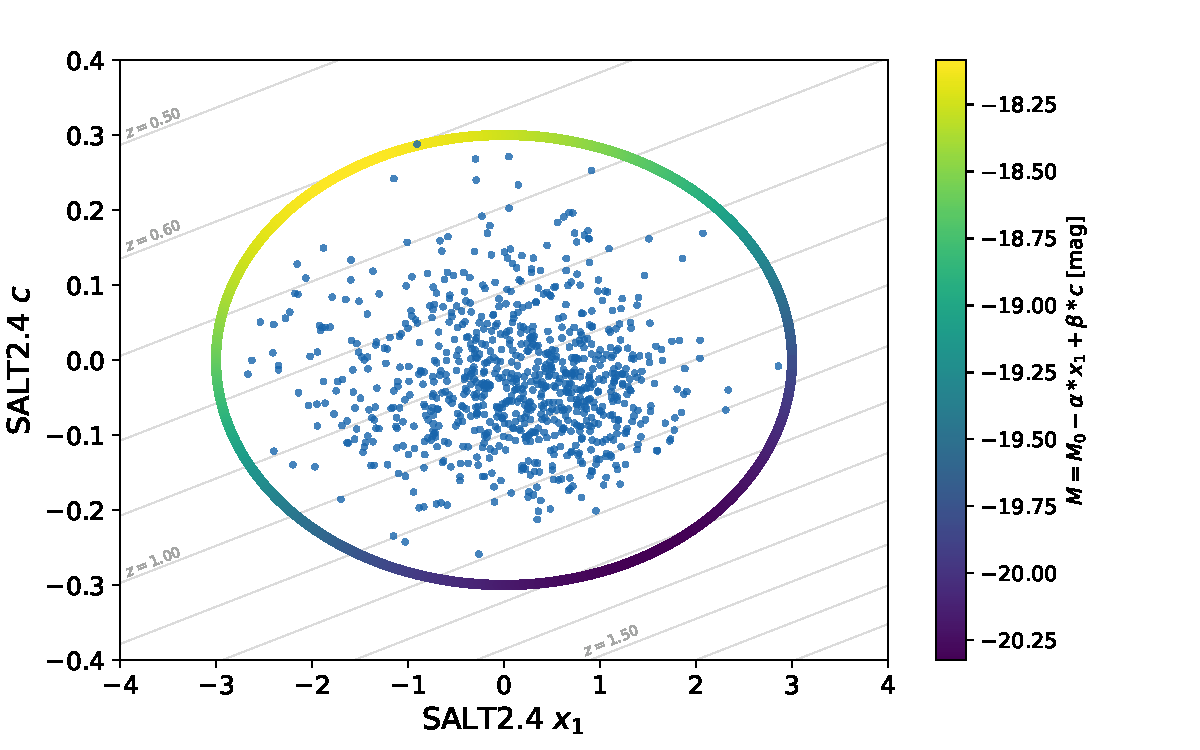
\includegraphics[width=0.95\linewidth]{Article_figures/zmax_maglim_snls.pdf}
    \caption{\textsc{\texttt{SALT2.4}} stretch and color lightcurve parameters
        of SNe~Ia from the SDSS, PS1 and SNLS samples from the pantheon catalog.
        The individual SN data are shown as blue dots and a 2D histogram is
        shown in gray to highlight point density. The ellipse
        ($x_1=\pm3\,\mathrm{;}\,c=\pm0.3$) is displayed, colored by the
        corresponding standardized absolute magnitude using the $\alpha$ and
        $\beta$ coefficients from \citep{scolnic2018a}. \nn{The lines represent
        the $(x_1, c)$ evolution for $m = m_{lim}$ in eq.~\ref{eq:m_lim},
    for $z=0.60$ and $z=0.70$ using SNLS's $m_{lim}$ of $24.8\,$mag. The data
    above these lines are those for which $m > m_{lim}$, meaning they can't be
    observed.}}
    \label{fig:maglim}
\end{figure}

SNLS typically acquires SNe~Ia in the redshift range $0.4<z<0.8$. At these
redshifts the rest-frame Bessel-B band roughly corresponds to the SNLS-$i$
filter that has a 24.8 mag $5\sigma$
depth\footnote{\href{https://www.cfht.hawaii.edu/Science/CFHTLS/cfhtlsfinalreleaseexecsummary.html}{CFHT
final release website.}}. This converts to a $z_{lim}=0.60$, in perfect
agreement with \cite{neill2006}, \cite{perrett2010} and \cite{bazin2011}.
Similarly, PS1 observes SNe~Ia in the range $0.2<z<0.4$, their $g$-band
$5\sigma$ depth is 23.1 mag \citep{rest2014}, which yields to $z_{lim}=0.30$ in
agreement with, e.g., Figure~6 of \cite{scolnic2018a}. This figure could also
suggest a more conservative $z_{lim}$ of 0.27; both will be considered as
discussed below.  In similar redshift range, SDSS has a limiting magnitude of
22.5 \citep{dilday2008,sako2008}, which would lead to a $z_{lim}=0.24$. However,
the SDSS surveys were more sensitive to limited spectroscopic resources.
\cite{kessler2009} \nn{pointed out} that during year-1 of SDSS, SNe~Ia with
$r-mag<20.5$ were favored for spectroscopic follow up, corresponding to the
redshift cut at $0.15$. For the rest of the SDSS survey, additional
spectroscopic resources were used, such that \cite{kessler2009} and
\cite{dilday2008} show a relative completeness up to $z_{lim}=0.2$. Following
these analyses we will use $z_{lim}=0.2$ as the baseline SDSS redshift limit for
the rest of \nn{this study}. For the rest of the analysis, we will consider both
cases, the \nn{aforementioned} redshift limits as well as more conservative cuts
for each of these surveys, namely $z_{lim}=0.15$ for SDSS, $z_{lim}=0.27$ for
PS1 and $z_{lim}=0.55$ for SNLS (following Fig.~14 of \citealt{perrett2010}).

The complete sample selection is summarized table~\ref{tab:sample} and the
redshift distribution of these three surveys are shown in Fig.~\ref{fig:cuts}.
We see in this figure that the redshift limits we have selected roughly
correspond to the peak of these histograms\nn{. As the peaks indicate that we
are starting to miss the faintest SNe~Ia, it seems logical to have the redshift
cuts fall near said peaks.}

\begin{figure}
    \centering
    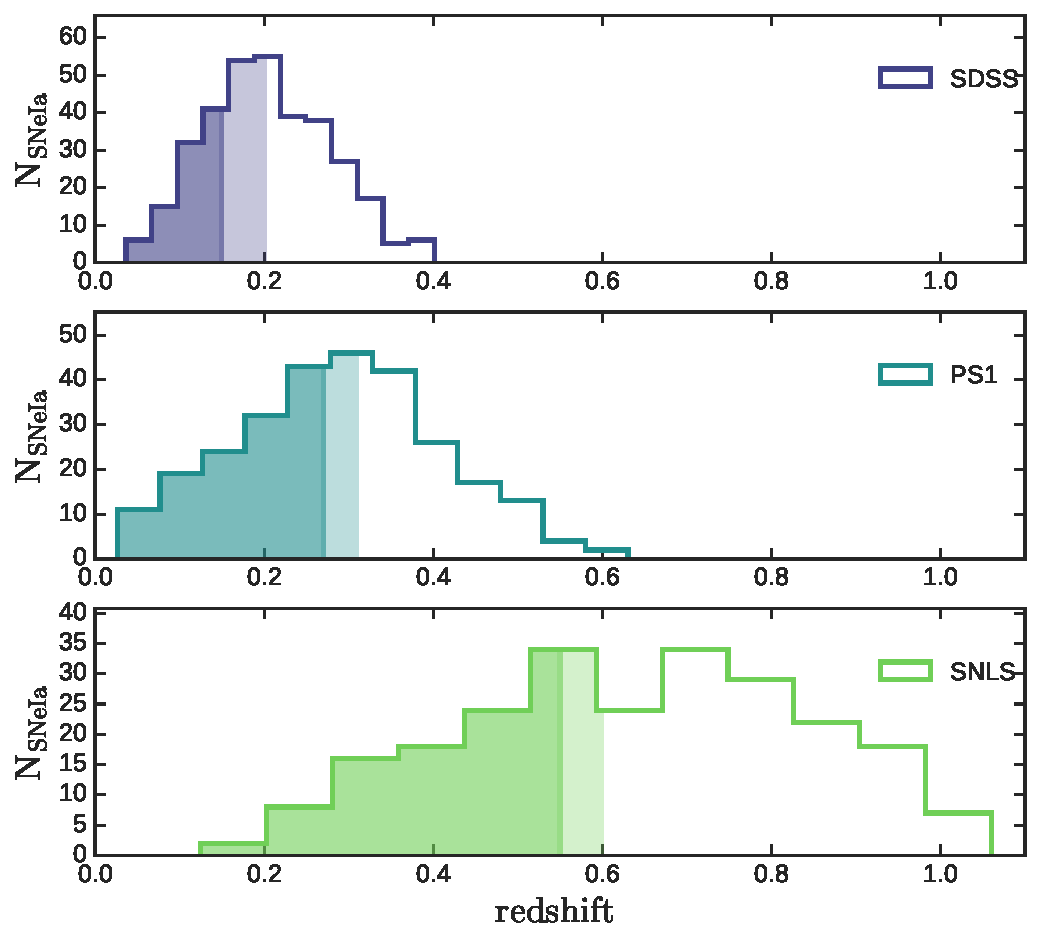
\includegraphics[width=0.9\linewidth]{Article_figures/hist_surveys_cuts.pdf}
    \caption{From top to bottom: histogram of SN~Ia redshifts for SDSS, PS1 and
    SNLS from the pantheon dataset, respectively. The colored part of the
distribution shows which SNe~Ia has been kept in our analysis for they are
supposedly free from selection bias (see section~\ref{sec:sample}). The
full(light) color responds to the conservative(nominal) cut.}
    \label{fig:cuts}
\end{figure}

In addition, we use the SNe~Ia from the Nearby Supernova Factory
\citep[SNfactory][]{aldering2004} published in \cite{rigault2018} and that have
been discovered from non-targeted searches (114 SNe~Ia, see their section~3 and
4.2.2). \nn{Their spectroscopic follow-up were only done on a redshift range of
$0.02<z<0.09$~\citep[as in ][]{rigault2018}, while the searches were much
deeper. As such, these SNe~Ia} should also be a random sampling of the underlying
SN population. The SNf data is particularly useful for studying SN property
drift as it enable us to have a large SN~Ia sample at $z<0.1$.  The HST sample
from Pantheon follows the same logic of having a search deeper than the
follow-up and we therefore kept it entirely \citep{FIND BACK THE REF}, see
table~\ref{tab:sample}.

\begin{table}
    \centering
    \caption{\nn{Source surveys and number of SNe~Ia used in our ''complete''
    sample. Conservative cuts are indicated in brackets.}}
    \label{tab:sample}
    \begin{tabular}{l c c}
    \hline\hline\\[-0.8em]
        Survey & z$_{lim}$ & N$_{\mathrm{SN}}$ \\[0.15em]
        \hline\\[-0.8em]
        SNf & -- & 114\\[0.30em]
        SDSS & 0.20(0.15) & 167(82)\\[0.30em]
        PS1 & 0.30(0.27) & 160(122)\\[0.30em]        
        SNLS & 0.60(0.55) & 102(78)\\[0.30em]
        HST & -- & 26\\[0.30em]
        Total & -- & 569(422)\\[0.30em]
        \hline
    \end{tabular}
\end{table}

%%%%%%%%%%%%%%%%%%%%%%%
%   LITERATURE        %
%%%%%%%%%%%%%%%%%%%%%%%
%\mri{COMPARE HERE WITH LITERATURE. E.G. FIG. 6 OF SCOLNIC 2018, PS zmax
%AROUND0.27}

%\mri{Perrett et al. 2010 | SNLS | zmax ="z $\sim$ 0.6"}

%\mri{Dilday et al. 2008 | SDSS | sure good at z<0.12, Fig. 10 suggest still
%okat z=0.2}

%\mri{Kessler 2009 "For the SDSS-II, the image-subtraction
%pipeline efficiency (	subtr) is complete up to a redshift of z ∼ 0.2"}

%\mri{Kesslet 2009 | "For the SDSS-II and SNLS samples, the cutoff redshifts are
%estimated to be 0.15 and 0.65, respectively."}
% ADDIND: PS cut from pantheon close to 0.27 see Fig. 6 of Scolnic 2018

%%%%%%%%%%%%%%%%%%%%%%%
%       INFO          %
%%%%%%%%%%%%%%%%%%%%%%%
%Fraction of random SDSS stretches being < mean_conservative =  0.299
%Fraction of random PS1 stretches being < mean_conservative =  0.254
%Fraction of random SNLS stretches being < mean_conservative =  0.417

\section{Modeling the redshift drift}
\label{sec:modeling}

In~\cite{rigault2018} we presented a modeling of the evolution of the fraction
of prompt and delayed SNe~Ia as a function of redshift following former work on
rates and delay time distributions \citep[e.g.,][]{mannucci2005,
scannapieco2005, sullivan2006, aubourg2008, childress2014, maozmannucci2014}.
In short, we assumed that the number of prompt SNe~Ia follows the star formation
activity \nn{(SFR)} in the Universe while the number of delayed SNe~Ia follows
the number of Gyr-old stars in the Universe, i.e. the stellar mass \nn{(M)}.
Hence, if we denote $\delta(z)$ (resp. $\psi(z)$) the fraction of young (resp.
old) SNe~Ia in the Universe as a function of redshift, then their ratio
$\delta/\psi$ is expected to follow the evolution of the specific star formation
rate \nn{(SFR/M)} which goes as $(1+z)^{2.8}$ until $z\sim2$
\citep[e.g.,][]{tasca2015}. Hence since \nn{$\delta(0.05) \sim \psi(0.05)$}
\citep{rigault2013,rigault2018,wiseman2020}, in agreement with rate expectations
\citep{mannucci2006,rodney2014}, \nn{and $\delta + \psi = 1$,} then we find in
\cite{rigault2018}:
\begin{align}
    \label{eq:delta}
    \delta(z) & = \left( K^{-1} \times (1+z)^{-2.8} +1 \right)^{-1}\,
    \mathrm{and}\\
    \psi(z) & = \left( K \times (1+z)^{+2.8} +1 \right)^{-1}
\end{align}
where $K=0.87$. This modelisation is comparable to the evolution predicted by
\cite{childress2014} based on SN rates in galaxies depending on their quenching
time as a function of their stellar mass.

\subsection{\nn{Base underlying distribution}}
\label{sec:basemodel}

\begin{figure*}
    \centering
    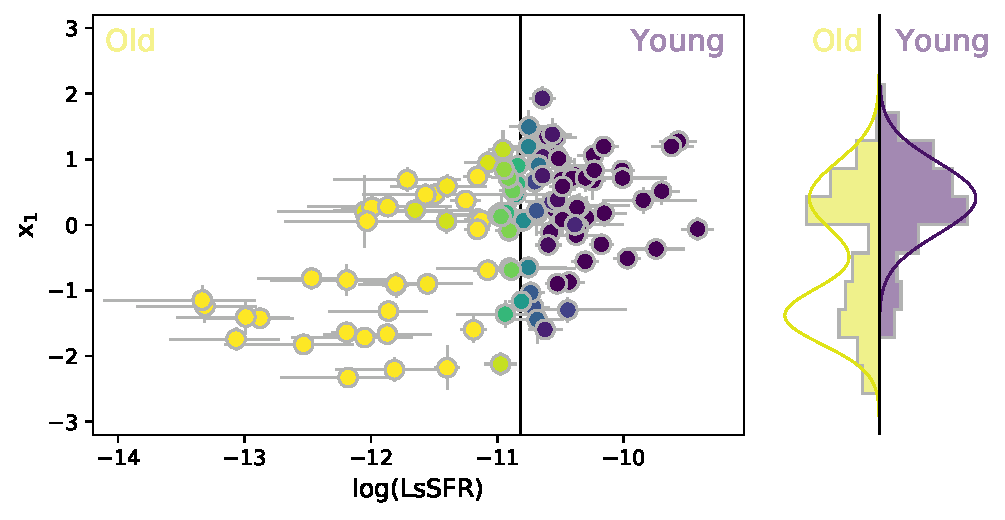
\includegraphics[width=0.8\linewidth]{Article_figures/model_base_hist.pdf}
    \caption{\textit{Main}: \textsc{\texttt{SALT2.4}} lightcurve stretch ($x_1$) as a function of
        the local specific star formation rate (LsSFR) for SNf data used in this
        analysis. The color corresponds to the probability for the SNe~Ia to be
        above $\log(\mathrm{LsSFR}=-10.82)$, which defines $p(y)$; see
        \cite{rigault2018}. \textit{Right}: histogram of $p(y)$-weighted
        marginalization of the SN stretch. On both panel, we illustrate the
        Base model fitted on the SNf data. The young and old population
        contributions are shown in purple and yellow, respectively.}
    \label{fig:stretchlssfr}
\end{figure*}

\nn{In~\cite{rigault2018} we presented the relation between SNe stretches and
LsSFR measurements, which trace progenitor age, from the SNf sample, and is
shown in Fig.~\ref{fig:stretchlssfr}}. To model the evolution of the SN stretch
as a function of redshift, given our aforementioned model of the evolution of
the fraction of young and old SNe~Ia with redshift, we need to model the SN
stretch distribution for each age subsample. Given the structure of the
stretch--LsSFR scatter plot shown in Fig.~\ref{fig:stretchlssfr}, we define our
model as follows: for the young population the underlying stretch distribution
is modeled as $\mathcal{N}(\mu_1, \sigma_1^2)$, i.e. a normal distribution
centered on $\mu_1$ with a $\sigma_1$ width; the old population stretch
distribution is modeled as $a\times \mathcal{N}(\mu_1, \sigma_1^2) + (1-a)\times
\mathcal{N}(\mu_2, \sigma_2^2)$, i.e. a gaussian mixture where one mode is the
same as the young population one. \nn{When combining our prediction of the
evolution of young SNe~Ia as a function of redshift (eq.~\ref{eq:delta}),
and the stretch distribution of both young and old SNe~Ia, our model for the
underlying distribution of stretch $X_1\left(z\right)$ as a function of
redshift is:}
\begin{align}
    \label{eq:stretchz}
    \nn{X_1\left(z \right) =
    } &\,\delta(z)\times\mathcal{N}(\mu_1,\sigma_1^2)\,+\nonumber\\
    (1-&\,\delta(z)) \times  \left[a\times\mathcal{N}(\mu_1,\sigma_1^2) +
    (1-a)\times\mathcal{N}(\mu_2,\sigma_2^2)\right]
\end{align}

The estimation of the 5 free parameters
($\theta\equiv{\mu_1,\mu_2,\sigma_1,\sigma_2,a}$) of the model is given by
minimizing a pseudo-$\chi^2$ $\mathcal{L}$ such that:

\begin{equation}
    \label{eq:likelihood}
    \mathcal{L} = -2 \sum_i \ln\left( \prob{x^{i}_{1}}{ \theta;
    \mathrm{d}x^{i}_{1}, \nn{y^i}}\right),
\end{equation}

\nn{where $i$ is the index of the SN~Ia, $x^{i}_{1}$, $\mathrm{d}x^{i}_{1}$ and
    $y^i$ are the \textsc{\texttt{SALT2.4}} stretch, error of the
    \textsc{\texttt{SALT2.4}} stretch and the probability that the SN is young,
    respectively. Depending on the data available, there are two ways to fit
these 5 free parameters}.

\subsubsection{\nn{Parameters estimation with LsSFR data}}
\label{sec:modelpy}

\nn{When using SNf data, we choose $y^i$ to be their given $p_y{}^i$, computed
from their LsSFR data (see Fig.~\ref{fig:stretchlssfr}). \nn{It represents the
probability to be above $\log(\mathrm{LsSFR} = -10.82)$.} Thus, we would have
$\mathcal{P}$ from eq.~\ref{eq:likelihood} to be}

\begin{align}
    \label{eq:likelihoodsnf}
    \prob{x^{i}_{1}}{\theta; \mathrm{d}x^{i}_{1}, p\nn{_y{}^i}} =
    \nn{p_y{}^i} \times &\mathcal{N}\left(\mu_1,
    \sqrt{\sigma_{1}^{2}+\mathrm{d}x^{i}_{1}{}^{2}}\right)(x^{i}_{1}) +
    \nonumber\\
        (1-\nn{p_y{}^i}) \times \nn{\bigg[} a \times &
        \mathcal{N}\left(\mu_1,
        \sqrt{\sigma_{1}^{2}+\mathrm{d}x^{i}_{1}{}^{2}}\right)(x^{i}_{1}) +
        \nonumber\\
     (1-a) \times &\mathcal{N}\left(\mu_2,
 \sqrt{\sigma_2{}^{2}+\mathrm{d}x^{i}_{1}{}^{2}}\right)(x^{i}_{1}) \nn{\bigg]}
\end{align}

In practice, since ''$a$'' is defined between 0 and 1, we fit for $\alpha$ such
that $a=\arctan(\alpha)/\pi+0.5$, which results into asymmetric error on $a$.
\mr{Results on fitting the SNf data with this model are shown
table~\ref{tab:modelresults} and illustrated in Fig.~\ref{fig:stretchlssfr}.}

\begin{table*}
    \centering
    \caption{Best fit values of the parameters for the Base stretch distribution
    model when applied to the SNf dataset only (114 SNe~Ia), the nominal 569
SN~Ia sample or the conservative one (422).}
    \label{tab:modelresults}
    \begin{tabular}{l c c c c c}
    \hline\hline\\[-0.8em]
        Sample & $\mu_1$  & $\sigma_1$ &$\mu_2$  & $\sigma_2$ & a \\[0.15em]
        \hline\\[-0.8em]
        SNf & $0.41 \pm 0.08$  & $0.55 \pm 0.06$ & $-1.38 \pm 0.10$ & $0.44 \pm 0.08$ & $0.48^{+0.08}_{-0.08}$ \\[0.15em]
        All & $0.37 \pm 0.05$  & $0.61 \pm 0.04$ & $-1.22 \pm 0.16$ & $0.56 \pm 0.10$ & $0.51^{+0.09}_{-0.10}$ \\[0.15em]
        All(cons) & $0.38 \pm 0.05$  & $0.60 \pm 0.04$ & $-1.26 \pm 0.13$ & $0.53 \pm 0.08$ & $0.47^{+0.09}_{-0.08}$ \\[0.15em]
        \hline
    \end{tabular}
\end{table*}

\subsubsection{Without LsSFR data}
\label{sec:modelnopy}

Given eq.~\ref{eq:stretchz}, we can extend the analysis to non-SNfactory sample
by fitting the free parameters of the model ($\theta\equiv{\mu_1, \mu_2,
\sigma_1, \sigma_2, a}$) assuming the evolution of the fraction of young SNe~Ia
as a function of redshift given by $\delta(z)$ and given, this time, $x_1^{i}$,
$\mathrm{d}x^{i}_{1}$ and $z^{i}$, the stretch, error on the stretch and
redshift of any given SN $i$. In practice, it means that we are still minimizing
for the same eq.~\ref{eq:likelihood}, but \nn{using $y^i = \delta(z^i)$, which
is equivalent to replacing $p_y{}^i$ with $\delta(z^i)$ in
eq.~\ref{eq:likelihoodsnf}.}

\mr{For the rest of the analysis, we will therefore fit for
eq.~\ref{eq:likelihood} using \nn{$p_y{}^i$} --~the
probability for the SN $i$ to be young~-- when available (i.e. for SNf
dataset) and $\delta(z^{i})$ --~the expected fraction of young SNe~Ia at the
SN redshift $z^{i}$~-- otherwise.}

\mr{Results on fitting all the 569(422) SNe~Ia data (with conservative cuts)
with this model are given table~\ref{tab:modelresults} and illustrated in
Fig.~\ref{fig:modelall}. We see in this figure that the measured mean SN~Ia
stretch per bin of redshift follows our redshift drift modeling. That is, when
considering selection-bias free SN~Ia samples, SNe~Ia at higher redshift have on
average larger stretch ($0.34 \pm 0.10$ at $z\sim0.65$) than those at lower
redshift ($-0.17\pm 0.10$ at $z\sim0.05$). This is indeed what is expected if
old environments favor low SN stretch \citep[e.g.]{howell2007} \textit{and} if
the fraction of old SNe~Ia reduces as a function of redshift. See
section~\ref{sec:results} for a more quantitative discussion.}

\begin{figure*}
    \centering
    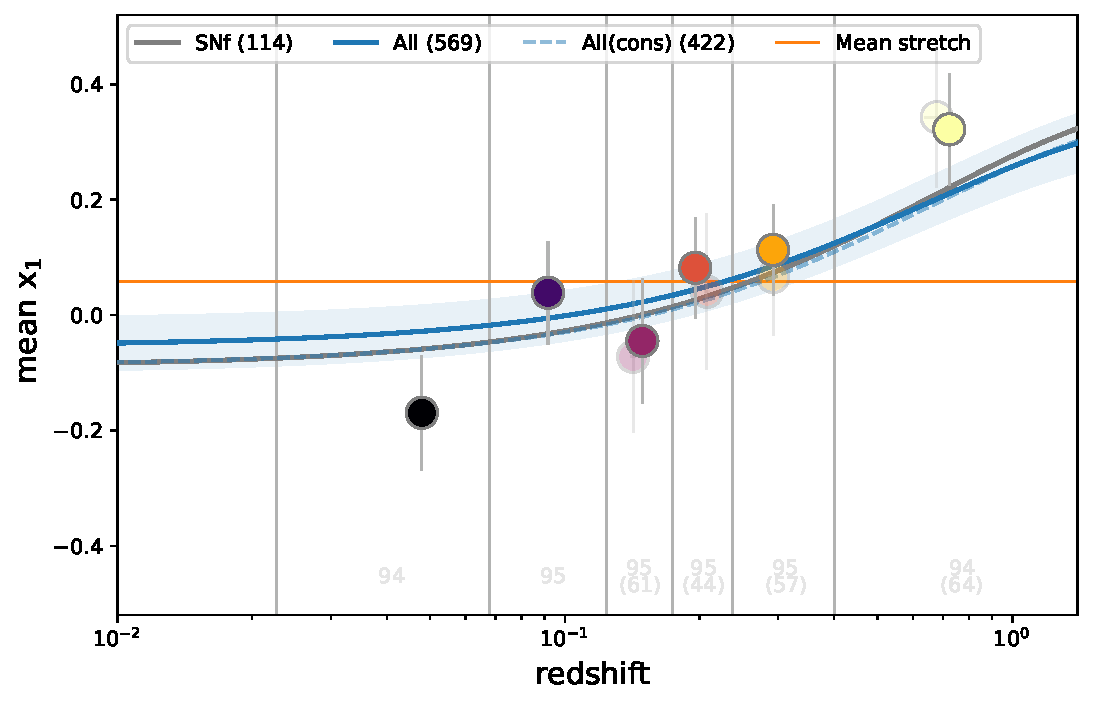
\includegraphics[width=0.7\linewidth]{Article_figures/stretchevol_all_vs_snf.pdf}
    \caption{Evolution of the mean SN \textsc{\texttt{SALT2.4}} stretch ($x_1$)
        as a function of redshift. Markers show the mean stretch measured in
        redshift bins of equal sample size indicated in light gray at the bottom
        of each redshift bins. Full and light markers are used when considering
        the nominal or the conservative sample, respectively, and are colored by
        their mean redshift. The orange horizontal line represents the mean
        redshift of the nominal sample illustrating the expectation if the SN
        stretch distribution is not drifting. Best fits of our Base drifting
        model are shown as blue, dashed-blue and gray, when fitted on the
    nominal, the conservative or the SNf dataset, respectively; all are similar.
The light-blue illustrates the amplitude of the error of the best fit model when
considering the nominal dataset.}
    \label{fig:modelall}
\end{figure*}

\subsection{Other modelings}
\label{sec:othermodel}

In section~\nn{\ref{sec:basemodel}} we have modeled the underlying stretch
distribution as a single gaussian for the young SNe Ia and a combination of two
gaussians for the old SNe Ia population, i.e., the same as the young-population
one plus another for the fast declining SNe~Ia that seem to only exist in old
populations. This is our “Base” model.

\cite{howell2007} used a simpler modelisation: a single gaussian for each age
sub-group. To test \nn{different modeling choices}, we have implemented a suite
of extra parametrisation that we also fit to the data following the procedure
described section~\ref{sec:modelnopy}. 

%Namely we consider:
%\begin{itemize}
 %   \item “Base$+(\mu_1^{\mathrm{O}}, \sigma_1^{\mathrm{O}})$”: Base model but where the high-stretch Gaussian of the old population is not set as that of the young population (+2 degrees of freedom);
 %   \item “Base$-(\sigma_2)$”: Base model but where $\sigma_2$ is fixed at the same value as $\sigma_1$ (-1 degree of freedom);
 %   \item “Howell”: one single Gaussian per age group as in \cite{howell2007}.
%\end{itemize}

\nn{We thus consider a model ''Howell+drift'', with one single gaussian per age
group as in \citet{howell2007}}. In addition, since we aim at probing the SN
redshift drift, we are also fitting the ''Base'' model and \nn{this
aforementioned extension} by fixing the population drift parameter $\delta(z)$
to a free parameter constant $\delta(z)=f$. 

We are also considering alternative non-drifting models, and notably the one
developed for the Beam with Bias Correction \cite[BBC,][]{scolnic2016,
kessler2017}, currently used by all recent SN Cosmological analyses
\cite[e.g.][]{scolnic2018a, descosmopaper2019, riess2016, riess2019} to account
for Malmquist biases. The BBC formalism assumes sample-based (hence
non-drifting) asymmetric Gaussian distributions ($\mathcal{N}\left(\mu,
\sigma^{-}{}^2\, \mathrm{if}\,x_1<\mu\,\mathrm{else}\, \sigma^{+}\right)$). The
idea behind the sample-based approach is twofold: (1) Malmquist biases are
driven by survey properties and (2) because current surveys cover limited
redshift ranges, doing so contains some potential redshift evolution information
\citep{scolnic2016, scolnic2018a}. See further discussion concerning the BBC
modeling in section~\ref{sec:bbc}. For the sake of the comparison, we are also
running Gaussian and asymmetric Gaussian non-drifting models. 

The ability of these models to explain the data is detailed in
section~\ref{sec:results}.

\section{Results}
\label{sec:results}
We applied each model on both the conservative and non-conservative samples (cf.
section \ref{sec:sample}). Because the models presented
section~\ref{sec:modeling} have various degrees of freedom, we use the Akaike
Information Criterion (AIC) \citep{burnham2004} to compare them. This estimator
penalizes extra degrees of freedom to avoid over-fitting the data. It is defined
as follow:
\begin{equation}
    \nn{\mathrm{AIC} = 2k - 2\ln L}
\end{equation}
where $k$ is the number of free parameters and \nn{$-2\ln L = \mathcal{L}$} is
the pseudo-$\chi^2$ defined eq.~\eqref{eq:likelihood}. The \nn{reference} model
is the one with the smaller AIC and the probability for another model to be at
least as representative of the data as this one is given by:
\begin{equation}
    p(\mathrm{other} \geq \mathrm{ref}) =
    \exp\left(\Delta\mathrm{AIC}/2\right)
\end{equation}
Results are presented in table \ref{tab:comp} and are illustrated
Fig.~\ref{fig:mod_comp}.

\begin{table*}
    \centering
    \caption{Comparison of the relative ability for a model to describe the data
        using AIC criterion. See the model definition
        section~\ref{sec:modeling}. The drift column indicates if the model
        contains the age-drifting model ($\delta(z)$) or not (f, i.e.
        non-drifting). The BBC modeling is sample based which somewhat contains
        redshift dependency information. $\mathcal{L}$ is the pseudo-$\chi^{2}$
        defined eq.~\ref{eq:likelihood} and Proba is the probability that a
        model is at least as good as the reference model to describe the data.
    See also Fig.~\ref{fig:mod_comp}.}
    \label{tab:comp}
    \begin{tabular}{c c c  |c c c c|  c c c c}\hline\hline\\[-0.8em]
        & & & \multicolumn{4}{|c}{All SNe~Ia (569)} & \multicolumn{4}{|c}{All SNe~Ia (conservative; 422)} \\
        %\cline{2-6}
        Name & drift & Free param &
        $\mathcal{L}$ & $\mathrm{AIC}$ & $\Delta \mathrm{AIC}$ & Proba & $\mathcal{L}$ & $\mathrm{AIC}$ & $\Delta \mathrm{AIC}$ & Proba \\[0.15em]
        \hline\\[-0.8em]

        Base & $\delta(z)$ & 5
        & 1456.7 & 1466.7 & -- & --
        & 1079.5 & 1089.5 & -- & --\\[0.15em]

        Howell & $\delta(z)$ & 4
        & 1463.3 & 1471.3 & -4.6 & $1.0\times10^{-1}$
        & 1088.2 & 1096.2 & -6.7 & $3.4\times10^{-2}$\\[0.15em]

        Asymmetric & -- & 3
        & 1485.2 & 1491.2 & -24.5 & $4.7\times10^{-6}$
        & 1101.3 & 1107.3 & -17.8 & $1.4\times10^{-4}$\\[0.15em]

        Howell & $f$ & 5
        & 1484.2 & 1494.2 & -27.5 & $1.0\times10^{-6}$
        & 1101.2 & 1111.2 & -21.7 & $1.9\times10^{-5}$\\[0.15em]

        Base & $f$ & 6
        & 1484.2 & 1496.2 & -29.5 & $3.9\times10^{-7}$
        & 1101.2 & 1113.2 & -23.7 & $7.1\times10^{-6}$\\[0.15em]

        BBC-modeling & per sample & 3x5
        & 1468.2 & 1498.2 & -31.5 & $1.5\times10^{-7}$
        & 1083.6 & 1113.6 & -24.1 & $5.7\times10^{-6}$\\[0.15em]

        Gaussian & -- & 2
        & 1521.8 & 1525.8 & -59.1 & $1.5\times10^{-13}$
        & 1142.6 & 1146.6 & -57.1 & $4.0\times10^{-13}$ \\\hline\hline
    \end{tabular}
\end{table*}

\begin{figure}
    \centering
    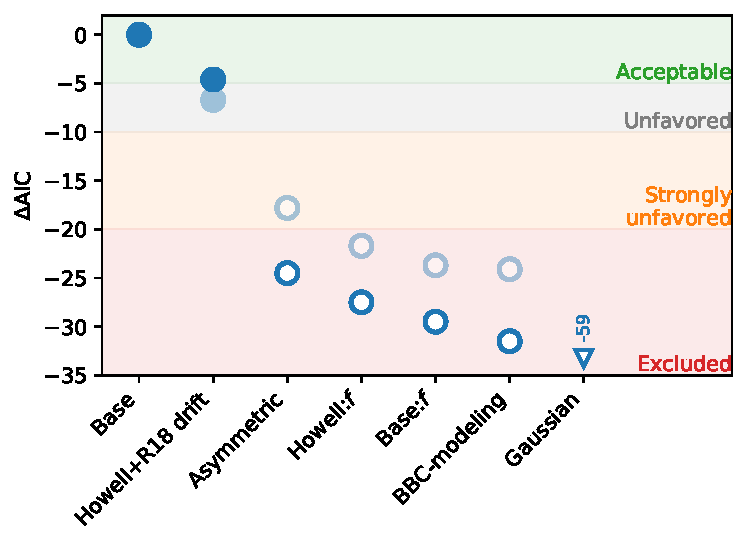
\includegraphics[width=\linewidth]{Article_figures/mod_comp.pdf}
    \caption{$\Delta$AIC between the reference model and the other considered
    models(see also table~\ref{tab:comp}). The full and open blue markers
correspond to model with and without redshift drift, respectively. Light markers
show the results when this analysis is done on the conservative sample.
Color-bands illustrate the validity of the models, from Acceptable to Excluded,
see inside text. All non-drifting models are excluded.}
    \label{fig:mod_comp}
\end{figure}

\mr{We find that underlying stretch distributions with no redshift drift are all
    excluded to describe the data as well as the Base redshift model. In fact,
    the best non drifting model (Asymmetric) has $2\times10^{-4}\%$ of chance to
    describe the data as well as Base. This is visible fig~\ref{fig:modelall}
    where the mean stretches per bin of redshift of equal sample size suggest a
    redshift evolution following our Base model --~fitted either on SNf, on the
    nominal 569 SNe~Ia dataset or the conservative one~-- rather than having a
constant mean value.}

\mr{As just mentioned, the \nn{reference model is Base}, but we also implemented
    a Base$-(\sigma_2)$ model, where both the low-stretch (mode 2 that only
    exists in old environments) and high-stretch (mode 1 that exists in all
    environments) normal distributions share the same width. It is marginally
    better than the Base model where both distributions have their own
    \nn{dispersion} ($\Delta \mathrm{AIC}<2$). Similarly, letting the
    high-stretch distribution to vary between the young and the old population
    (\nn{model we call} Base$+(\mu_1^{\mathrm{O}}, \sigma_1^{\mathrm{O}})$) only
    marginally improves the fit ($\Delta\mathcal{L}=3.6$ in comparison to Base)
    at a cost of 2 more degrees of freedom, making this mode less likely. This
    suggests that, indeed, the high-stretch mode (mode 1) exists in all kind of
    age-populations. We also remark that considering the stretch distribution of
    each age-population as independent normal distributions, as suggested by
\cite{howell2007}, is \nn{significantly disfavored}.}

\mr{Our results strongly suggest that the underlying distribution of SN~Ia
    stretch evolves as a function of redshift. Our redshift drift modeling
    presented section~\ref{sec:modeling} is a much better representation of the
    pantheon data (see section~\ref{sec:sample}) than any non-drifting models,
    including the sample-based BBC one. Considering or not the conservative
sample has no effect on our conclusion as illustrated Fig.~\ref{fig:modelall}
and presented table~\ref{tab:comp}.}

\mr{To the best of our knowledge, the SN~Ia stretch redshift drift has never
    been explicitly accounted for in cosmological analyses. Not doing so is a
    second order issue for SN cosmology as it only affects the way one does
    Malmquist bias correction. Indeed, as long as the Phillip's relation
    standardization parameter $\alpha$ is not redshift dependent (study behind
    the scope of this paper, but see e.g. \citealt{scolnic2018a}), if a sample
    is free from selection effects, the stretch-corrected SNe~Ia magnitudes used
    for cosmology are blind to the underlying stretch distribution.  However,
    since the first missed SNe~Ia are the faintest, which are also those with
    the lowest stretch, once we include SNe~Ia affected by selection effects we
    need to account for the fact that only the brightest SNe~Ia exist in the
    low-stretch end of the sample after standardization. The modeling of the SN
    stretch then enters the analysis to understand which SNe~Ia are missing
given the selection functions to mimic a selection-bias free sample.}

\mr{The state-of-the-art tool for doing so is the BBC described in
    \cite{scolnic2016} and \cite{kessler2017}, which is used in all recent SN
    Cosmological analyses \citep{jones2018b, scolnic2018a, brout2019,
    descosmopaper2019} including the direct measurement of H$_0$
\citep{riess2016,riess2019}. As already discussed, it currently assumes an
asymmetric stretch distribution per sample. \nn{A more detailed discussion on
this modeling is presented section \ref{sec:bbc}.}}

\section{\nn{BBC discussion}}
\label{sec:bbc}
\mr{Surprisingly, the BBC technique, which assumes an individual asymmetric
    distribution per sample \citep{scolnic2016,kessler2017}, is one of the worst
    modelisation. While its pseudo-$\chi^{2}$ $\mathcal{L}$ is the best of all
    the non-drift model, but still $\Delta \mathcal{L}=-11.5$ worse than our
    best model, it is penalized by requiring 15 free parameters, 3 per sample.
    \citet[][section~2]{scolnic2016} and \citet[][section~5.4]{scolnic2018a}
    highlighted that, because current surveys span limited redshift ranges, the
    per sample approach somewhat accounts for unmodeled redshift drifts. We
    stress here that, as measurements of modern surveys cover larger redshift
    ranges to reduce calibration systematic  uncertainties, this is becoming
    less true, notably for PS1, DES and, soon, LSST. Already with the current
    surveys, the BBC sample-based technique is excluded to be an as good
    representation of the data as our best model ($p=4\times 10^{-8}$). A more
    detailed discussion of the consequence of this results for cosmology follows
in section~\ref{sec:bbc}}

\mr{We report in table~\ref{tab:bbc} the samples' $\sigma^-$, $\sigma^+$ and
    $\mu^0$ that we find in close agreement with \cite{scolnic2016} for SNLS and
    SDSS and with \cite{scolnic2018a} for PS1. This validates \nn{the} somewhat
    simple construction of our selection-bias free sample, see
    section~\ref{sec:sample}. If we were to use the \cite{scolnic2016} and
    \cite{scolnic2018a} best fit values for SNLS, SDSS and PS1, respectively,
    the $\Delta\mathrm{AIC}$ between our Base drifting model and the BBC
    modeling would go from -32 to -47. \nn{It would seem that our minimization
    of these parameters is closer to our Base model than theirs}. Furthermore,
    fixing the Base model parameters to those derived using SNf data only (top
    row table.~\ref{tab:modelresults}) and using the BBC parameters from the
    aforementioned literature for PS1, SDSS and SNLS, we find
    $\Delta\mathrm{AIC}=-31.7$. Removing the SNf data reduces this difference to
    $\Delta\mathrm{AIC}=-5$. Such a reduction is expected for two reasons.
    First, it removes the nearby SNe~Ia, and thereby significantly reduces the
    redshift level arm to probe the impact of potential redshift drifts.
    Second, the SNf data are better at discriminating the individual stretch
    distributions by age since the probability for a SN to be young $p_y{}^i$ is
    known while other samples rely on $\delta(z^i)$ which only is the fraction
    of young SNe~Ia at the SN redshift, i.e. a probabilistic proxy for
    $p_y{}^i$. While in any case the Base-model is favored, the relative weight
    of a SNf sample highlights the importance of adding non-targeted nearby
surveys, such as the Zwicky Transient Facility \cite[ZTF,][]{bellm2019,
graham2019} to unambiguously confirm our result.}

%Using S18/SK16 values of \sigma_-, \sigma_+ and \mu_0, we find that SDSS, PS1 and SNLS's $\mathcal{L}$ to be 457.9, 397.6 and 254.5 respectively, and their AIC to be 464.0, 403.7 and 260.8 respectively, systematically higher than those we find in this study (see table \ref{tab:bbc_comp}).

\begin{table}
    \centering
    \caption{Best fit parameters for our sample-based asymmetric modeling of the
    underlying stretch distribution.}
    \label{tab:bbc}
    \begin{tabular}{c c c c c c c}\hline\hline\\[-0.8em]
    Asymmetric & $\sigma^-$ & $\sigma^+$ & $\mu^0$ \\\hline\\[-0.8em]
    SNf &  1.34 $\pm$ 0.13 & 0.41 $\pm$ 0.10 & 0.68 $\pm$ 0.15\\[0.15em]
    SDSS & 1.31 $\pm$ 0.11 & 0.42 $\pm$ 0.09 & 0.72 $\pm$ 0.13 \\[0.15em]
    PS1 &  1.01 $\pm$ 0.11 & 0.52 $\pm$ 0.12 & 0.38 $\pm$ 0.16 \\[0.15em]
    SNLS & 1.41 $\pm$ 0.13 & 0.15 $\pm$ 0.13 & 1.22 $\pm$ 0.15 \\[0.15em]
    HST &  0.76 $\pm$ 0.36 & 0.79 $\pm$ 0.35 & 0.11 $\pm$ 0.44 \\\hline\hline
    \end{tabular}
\end{table}

\begin{figure}
    \centering
    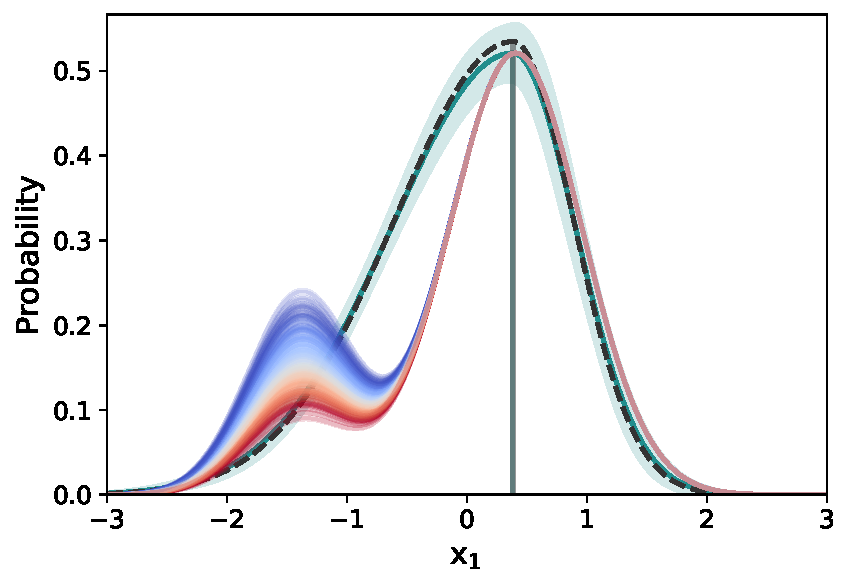
\includegraphics[width=\linewidth]{Article_figures/bbc_comp_PS1.pdf}
    \caption{Underlying SN \textsc{\texttt{SALT2.4}} stretch ($x_1$)
        distributions for the PS1 sample. The Green line(band) shows our best
        fitted asymmetric Gaussian distribution (its error) mimicking the BBC
        approach. The dashed line shows the noe estimated by
    \cite{scolnic2018a}. The blue to red curves display our Base drifting
stretch model estimated at each PS SN redshift; bluer for lower redshifts.}
    \label{fig:bbc_pdf_ps1}
\end{figure}

\mr{We illustrate Fig.~\ref{fig:bbc_pdf_ps1} the prediction difference in the
underlying stretch distribution between the BBC modeling and our Base drifting
model for the PS1 sample. By definition, our model is bimodal and the relative
amplitude of each mode depends on the fraction of old SNe~Ia in the sample
--~the highest the fraction of old SNe~Ia, the highest the amplitude of the
low-stretch mode~-- and is therefore redshift dependent. As expected the two
approaches strongly differ in modeling the negative part of the SN stretch
distribution. The BBC asymmetric distribution goes in the middle of the bimodal
distribution, largely over-estimating the number of SNe~Ia at $x_1\sim-0.7$ and
largely under-estimating it at $x_1\sim-1.7$ for typical PS1 SN redshifts. This
means that the bias-correction of the individual SN stretch
$\overline{\delta}_{x_1}$ \citep{kessler2017} and consequently the magnitude
bias correction $\mu_B$ is most likely inaccurate. However, given the complexity
of the BBC analysis, a full study using our Base model given
eq.~\ref{eq:stretchz} in place of the sample-based asymmetric modeling would be
necessary to have an exact understanding of the effect this inaccurate modeling
has on cosmology.}

\mr{Nonetheless, to have a rough estimation of the expected amplitude of the
effect, we show Fig.~\ref{fig:magdrift} the difference of mean stretch
correction $\alpha\times\left(\langle x_1 \rangle_{\mathrm{BBC}} - \langle x_1
\rangle_{\mathrm{Base}}\right)$ as a function of redshift, using $\alpha=0.156$
from \cite{scolnic2018a}. We see in this figure that the amplitude of the
magnitude bias caused by an accurate modeling of the underlying stretch
distribution is of the order of few tens of millimag, which is the typical scale
that exotic forms of dark energy could have on $\mu(z)$. In the era of modern
cosmology where we aim at probing $w_0$ at a sub-percent and $w_a$ at a few
percent \citep[e.g.,][]{lsstpaper}, it is therefore of paramount importance to
further understand the exact modeling of the lightcurve parameters and
especially their potential redshift drift; see also discussions about the impact
of stretch and color distribution modeling for cosmology in \citealt{rubin2015}
and \citealt{rubin2016}.}

\begin{figure}
    \centering
    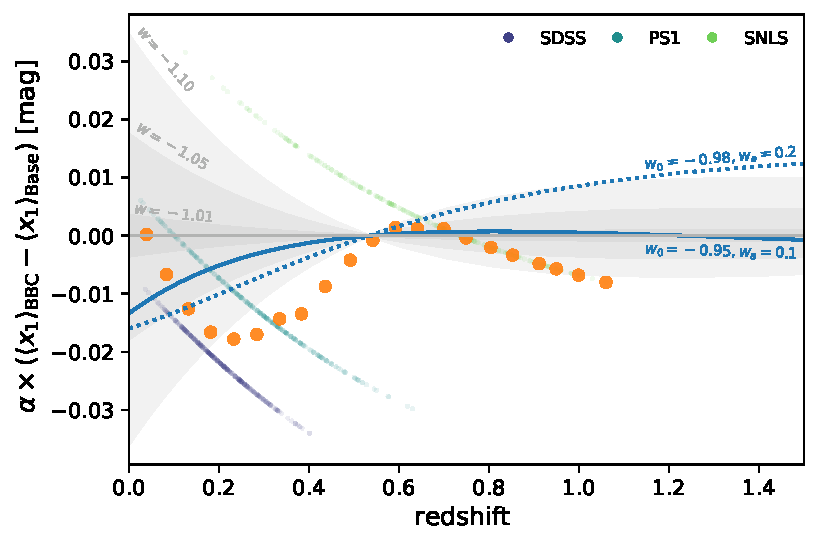
\includegraphics[width=\linewidth]{Article_figures/BBC_distmod_w0wa.pdf}
    \caption{Difference of mean stretch standardization (in mag) between the BBC
        algorithm used in \cite{scolnic2018a} and our Base drifting model.
        \nn{The small colored points show the SDSS, PS1 and SNLS evolution,
            while the orange markers represent their mean evolution in 30
            regular redshift bins.} For comparison, we show in gray bands the
            expected magnitude difference between $\Lambda$CDM and $w$CDM
            cosmologies ($w=-1\pm 10,\,5\,\mathrm{and}\,1\%$) or, in orange,
            more exotic $w_0,w_a$CDM examples. This figure illustrates that the
            amplitude of the potential magnitude bias caused by inaccurate
        modeling of the underlying stretch distribution is comparable to the
    observational effect of exotic form of dark energy.}
    \label{fig:magdrift}
\end{figure}

\section{Conclusion}
\label{sec:ccl}
We have presented a study of the drift of the underlying SNe~Ia stretch
distribution as a function of redshift. We used SNe~Ia from magnitude-limited
surveys from the pantheon dataset \citep[][SDSS, PS1 and SNLS]{scolnic2018a} as
well as HST to which we added SNfactory data from \cite{rigault2018} for the
low-redshift bin. We only considered the supernovae that have been discovered
in redshift ranges of each surveys where selection effect are negligible. This
way the observed SNe~Ia stretch are random sampling of the true underlying
distribution. This corresponds to 569 SNe~Ia (422 when considering more
conservative cuts).

Following observations made in \cite{rigault2018} we introduced a redshift drift
modeling that depends on the expected fraction of young and old SNe~Ia as a
function of redshift, each age-population having its own underlying stretch
distribution. We studied various suites of distribution as well as non-drifting
modeling. We also closely studied the stretch distribution modeling made in
current version of the BCC algorithm used for Malmquist bias correction by all
recent Dark energy or Hubble constant cosmological analyses. 

Our conclusions are the following:
\begin{enumerate}

    \item Non-drifting models are excluded to be as good descriptions of the
        data \nn{as} our Base modeling. This model assumes that: (1) the young
        population has an unimodal Gaussian stretch distribution while the old
        population stretch one is bimodal, one mode being the young one; (2) the
        evolution of the relative fraction of young and old SNe~Ia follows the
        prediction made in \cite{rigault2018}. 

    \item Given 1. we conclude that the SNe~Ia is indeed drifting, as already
        suggested by \citep[e.g.][]{howell2007}. 

    \item The BBC approach, which assumes each survey to have its own asymmetric
        Gaussian distribution, is excluded to be an as good description of the
        data as our drifting model ($p=4\times10^{-8}$). Hence, the BBC
        sample-based approach does not accurately account for redshift drift as
        suggested by \cite{scolnic2016} and \cite{scolnic2018a}.

    \item An inaccurate underlying stretch distribution modeling is estimated to
        bias the mean standardized SNe~Ia on the order of a few percent, which
        is comparable in scale to the observational signature of exotic forms of
        dark energy.

    \item We suggest to use the following stretch population modeling:
    \begin{align}
    \label{eqconclusion:stretchz}
        \Delta\left(x_1\,|\,z \right) =
        &\,\delta(z)\times\mathcal{N}(\mu_1,\sigma_1)\,+\nonumber\\
        (1-&\,\delta(z)) \times  \left[a\times\mathcal{N}(\mu_1,\sigma_1) +
        (1-a)\times\mathcal{N}(\mu_2,\sigma_2)\right]\nonumber
    \end{align}
    with: $a=0.50$, $\mu_1=0.37$, $\mu_2=-1.22$, $\sigma_1=0.61$,
    $\sigma_2=0.56$, see table~\ref{tab:modelresults} and using the
    age-population drift modelization $\delta(z)$ defined in \cite{rigault2018}
    with $K=0.87$:
    \begin{align}
        \delta(z) & = \left( K^{-1} \times (1+z)^{-2.8} +1 \right)^{-1}\nonumber
    \end{align}
\end{enumerate}

\begin{acknowledgements}
    This project has received funding from the European Research Council (ERC)
    under the European Union's Horizon 2020 research and innovation programme
    (grant agreement n 759194 - USNAC).
    % How has received that support for this project ? 
    %Support has been provided by the Institut Universitaire de France, the CNES, and the region Auvergne-Rhone-Alpes.
\end{acknowledgements}

\bibliographystyle{aa} % style aa.bst
\begin{thebibliography}{} 
% A
\bibitem[Abbott et al.(2018)]{abbott2018} Abbott, T.~M.~C., Abdalla, F.~B., Alarcon, A., et al.\ 2018, \prd, 98, 043526

\bibitem[Abbott et al.(2019)]{descosmopaper2019} Abbott, T.~M.~C., Allam, S., Andersen, P., et al.\ 2019, \apjl, 872, L30

\bibitem[Aldering(2004)]{aldering2004} Aldering, G.\ 2004, APS April Meeting Abstracts 2004, V4.003

\bibitem[Astier et al.(2006)]{astier2006} Astier, P., Guy, J., Regnault, N., et al.\ 2006, \aap, 447, 31


\bibitem[Ata et al.(2017)]{ata2017} Ata, M., Kitaura, F.-S., Chuang, C.-H., et al.\ 2017, \mnras, 467, 3993

\bibitem[Aubourg et al.(2008)]{aubourg2008} Aubourg, {\'E}.,
  Tojeiro, R., Jimenez, R., et al.\ 2008, \aap, 492, 631 


% B
\bibitem[Bazin et al.(2011)]{bazin2011} Bazin, G., Ruhlmann-Kleider, V., Palanque-Delabrouille, N., et al.\ 2011, \aap, 534, A43

\bibitem[Bellm et al.(2019)]{bellm2019} Bellm, E.~C., Kulkarni, S.~R., Graham, M.~J., et al.\ 2019, \pasp, 131, 018002

\bibitem[Betoule et al.(2014)]{betoule2014} Betoule, M., Kessler, R., Guy, J., et al.\ 2014, \aap, 568, A22

\bibitem[Brout et al.(2019)]{brout2019} Brout, D., Scolnic, D., Kessler, R., et al.\ 2019, \apj, 874, 150

\bibitem[Burnham \& Anderson(2004)]{burnham2004} Burnham, K., Anderson, D., \
2004, Sociological Methods \& Research, 33, 2

% C
\bibitem[Campbell et al.(2013)]{campbell2013} Campbell, H., D'Andrea, C.~B., Nichol, R.~C., et al.\ 2013, \apj, 763, 88


\bibitem[Chabanier et al.(2019)]{chabanier2019} Chabanier, S., Millea, M., \& Palanque-Delabrouille, N.\ 2019, \mnras, 489, 2247

\bibitem[Childress et al.(2013)]{childress2013} Childress, M., Aldering, G., Antilogus, P., et al.\ 2013, \apj, 770, 108

\bibitem[Childress et al.(2014)]{childress2014} Childress, M.~J., Wolf, C., \& Zahid, H.~J.\ 2014, \mnras, 445, 1898


\bibitem[Coles, \& Jones(1991)]{coles1991} Coles, P., \& Jones, B.\ 1991, \mnras, 248, 1

%\bibitem[Conley et al.(2011)]{conley2011} Conley, A., Guy, J., Sullivan, M., et al.\ 2011, \apjs, 192, 1


% D
\bibitem[D'Andrea et al.(2011)]{dandrea2011} D'Andrea, C.~B., Gupta, R.~R., Sako, M., et al.\ 2011, \apj, 743, 172

\bibitem[Dilday et al.(2008)]{dilday2008} Dilday, B., Kessler, R., Frieman, J.~A., et al.\ 2008, \apj, 682, 262


% E
% F
\bibitem[Feeney et al.(2019)]{feeney2019} Feeney, S.~M., Peiris, H.~V., Williamson, A.~R., et al.\ 2019, \prl, 122, 061105

\bibitem[Freedman et al.(2019)]{freedman2019} Freedman, W.~L., Madore, B.~F., Hatt, D., et al.\ 2019, \apj, 882, 34

\bibitem[Frieman et al.(2008)]{frieman2008} Frieman, J.~A., Bassett, B., Becker, A., et al.\ 2008, \aj, 135, 338


% G
\bibitem[Graham et al.(2019)]{graham2019} Graham, M.~J., Kulkarni, S.~R., Bellm, E.~C., et al.\ 2019, \pasp, 131, 078001

\bibitem[Gupta et al.(2011)]{gupta2011} Gupta, R.~R., D'Andrea, C.~B., Sako, M., et al.\ 2011, \apj, 740, 92

\bibitem[Guy et al.(2007)]{guy2007} Guy, J., Astier, P., Baumont, S., et al.\ 2007, \aap, 466, 11

%\bibitem[Guy et al.(2010)]{guy2010} Guy, J., Sullivan, M., Conley, A., et al.\ 2010, \aap, 523, A7

%\bibitem[Graziani et al.(2019)]{graziani2019} Graziani, R., Courtois, H.~M., Lavaux, G., et al.\ 2019, \mnras, 488, 5438

% H
\bibitem[Hamuy et al.(1996)]{hamuy1996} Hamuy, M., Phillips, M.~M., Suntzeff, N.~B., et al.\ 1996, \aj, 112, 2391

\bibitem[Hamuy et al.(2000)]{hamuy2000} Hamuy, M., Trager, S.~C., Pinto, P.~A., et al.\ 2000, \aj, 120, 1479

\bibitem[Howell et al.(2007)]{howell2007} Howell, D.~A., Sullivan, M., Conley, A., et al.\ 2007, \apjl, 667, L37

%\bibitem[Howell et al.(2009)]{howell2009} Howell, D.~A., Sullivan, M., Brown, E.~F., et al.\ 2009, \apj, 691, 661

% I 
% J
\bibitem[Jones et al.(2015)]{jones2015} Jones, D.~O., Riess, A.~G., \& Scolnic, D.~M.\ 2015, \apj, 812, 3
1

\bibitem[Jones et al.(2018)]{jones2018} Jones, D.~O., Riess, A.~G., Scolnic, D.~M., et al.\ 2018, \apj, 867, 108

\bibitem[Jones et al.(2018)b]{jones2018b} Jones, D.~O., Scolnic, D.~M., Riess, A.~G., et al.\ 2018, \apj, 857, 51

\bibitem[Jones et al.(2019)]{jones2019} Jones, D.~O., Scolnic, D.~M., Foley, R.~J., et al.\ 2019, \apj, 881, 19

% K
\bibitem[Kelly et al.(2010)]{kelly2010} Kelly, P.~L., Hicken, M., Burke, D.~L., et al.\ 2010, \apj, 715, 743

\bibitem[Kessler et al.(2009)]{kessler2009} Kessler, R., Becker, A.~C., Cinabro, D., et al.\ 2009, \apjs, 185, 32

\bibitem[Kessler \& Scolnic(2017)]{kessler2017} Kessler, R., \& Scolnic, D.\ 2017, \apj, 836, 56

\bibitem[Knox \& Millea(2019)]{knox2019} Knox, L., \& Millea, M.\ 2019, arXiv e-prints, arXiv:1908.03663

% L
\bibitem[Lampeitl et al.(2010)]{lampeitl2010} Lampeitl, H., Smith, M., Nichol, R.~C., et al.\ 2010, \apj, 722, 566

% M
\bibitem[Mannucci et al.(2005)]{mannucci2005} Mannucci, F.,
  Della Valle, M., Panagia, N., et al.\ 2005, \aap, 433, 807 
\bibitem[Mannucci et al.(2006)]{mannucci2006} Mannucci, F.,
  Della Valle, M., \& Panagia, N.\ 2006, \mnras, 370, 773 

\bibitem[Maoz et al.(2014)]{maozmannucci2014} Maoz, D., Mannucci,
  F., \& Nelemans, G.\ 2014, \araa, 52, 107 


% N
\bibitem[Neill et al.(2006)]{neill2006} Neill, J.~D., Sullivan, M., Balam, D., et al.\ 2006, \aj, 132, 1126

\bibitem[Neill et al.(2009)]{neill2009} Neill, J.~D., Sullivan, M., Howell, D.~A., et al.\ 2009, \apj, 707, 1449

% O
% P
\bibitem[Pan et al.(2014)]{pan2014} Pan, Y.-C., Sullivan, M., Maguire, K., et al.\ 2014, \mnras, 438, 1391

\bibitem[Perlmutter et al.(1999)]{perlmutter1999} Perlmutter, S., Aldering, G., Goldhaber, G., et al.\ 1999, \apj, 517, 565

\bibitem[Perrett et al.(2010)]{perrett2010} Perrett, K., Balam, D., Sullivan, M., et al.\ 2010, \aj, 140, 518

\bibitem[Planck Collaboration et al.(2016)]{planck2016} Planck Collaboration, Ade, P.~A.~R., Aghanim, N., et al.\ 2016, \aap, 594, A13

\bibitem[Poulin et al.(2019)]{poulin2019} Poulin, V., Smith, T.~L., Karwal, T., et al.\ 2019, \prl, 122, 221301

\bibitem[Planck Collaboration et al.(2018)]{planck2018} Planck Collaboration, Aghanim, N., Akrami, Y., et al.\ 2018, arXiv e-prints, arXiv:1807.06209

% Q
% R
\bibitem[Reid et al.(2019)]{reid2019} Reid, M.~J., Pesce, D.~W., \& Riess, A.~G.\ 2019, arXiv e-prints, arXiv:1908.05625

\bibitem[Rest et al.(2014)]{rest2014} Rest, A., Scolnic, D., Foley, R.~J., et al.\ 2014, \apj, 795, 44

\bibitem[Riess et al.(1998)]{riess1998} Riess, A.~G., Filippenko, A.~V., Challis, P., et al.\ 1998, \aj, 116, 1009

\bibitem[Riess et al.(2009)]{riess2009} Riess, A.~G., Macri, L., Casertano, S., et al.\ 2009, \apj, 699, 539

\bibitem[Riess et al.(2016)]{riess2016} Riess, A.~G., Macri, L.~M., Hoffmann, S.~L., et al.\ 2016, \apj, 826, 56

\bibitem[Riess et al.(2018)]{riess2018} Riess, A.~G., Casertano, S., Yuan, W., et al.\ 2018, \apj, 861, 126

\bibitem[Riess et al.(2019)]{riess2019} Riess, A.~G., Casertano, S., Yuan, W., et al.\ 2019, \apj, 876, 85

\bibitem[{Rigault {et~al.}(2013)}]{rigault2013}
Rigault, M., Copin, Y., Aldering, G., {et~al.} 2013, \aap, 560, A66

\bibitem[Rigault et al.(2015)]{rigault2015} Rigault, M., Aldering, G., Kowalski, M., et al.\ 2015, \apj, 802, 20

\bibitem[Rigault et al.(2018)]{rigault2018} Rigault, M.,
  Brinnel, V., Aldering, G., et al.\ 2018, arXiv:1806.03849

\bibitem[Rodney et al.(2014)]{rodney2014} Rodney, S.~A.,
  Riess, A.~G., Strolger, L.-G., et al.\ 2014, \aj, 148, 13 
  
\bibitem[Roman et al.(2018)]{roman2018} Roman, M., Hardin, D., Betoule, M., et al.\ 2018, \aap, 615, A68

\bibitem[Rose et al.(2019)]{rose2019} Rose, B.~M., Garnavich, P.~M., \& Berg, M.~A.\ 2019, \apj, 874, 32


\bibitem[Rubin et al.(2015)]{rubin2015} Rubin, D., Aldering, G., Barbary, K., et al.\ 2015, \apj, 813, 137

\bibitem[Rubin \& Hayden(2016)]{rubin2016} Rubin, D., \& Hayden, B.\ 2016, \apjl, 833, L30


% S
\bibitem[Sako et al.(2008)]{sako2008} Sako, M., Bassett, B., Becker, A., et al.\ 2008, \aj, 135, 348

\bibitem[Scannapieco \& Bildsten(2005)]{scannapieco2005} Scannapieco, E., \& Bildsten, L.\ 2005, \apjl, 629, L85 

\bibitem[Scolnic et al.(2014)]{scolnic2014} Scolnic, D., Rest, A., Riess, A., et al.\ 2014, \apj, 795, 45

\bibitem[Scolnic \& Kessler(2016)]{scolnic2016} Scolnic, D., \& Kessler, R.\ 2016, \apjl, 822, L35


\bibitem[Scolnic et al.(2018)]{scolnic2018a} Scolnic, D.~M., Jones, D.~O., Rest, A., et al.\ 2018a, \apj, 859, 101

\bibitem[Scolnic et al.(2018)]{scolnic2018b} Scolnic, D.~M., Lochner, M., Gris, P., et al.\ 2018, arXiv e-prints, arXiv:1812.00516

\bibitem[Scolnic et al.(2019)]{scolnicastro2020} Scolnic, D., Perlmutter, S., Aldering, G., et al.\ 2019, Astro2020: Decadal Survey on Astronomy and Astrophysics, 2020, 270

\bibitem[Sullivan et al.(2006)]{sullivan2006} Sullivan, M., Le  Borgne, D., Pritchet, C.~J., et al.\ 2006, \apj, 648, 868 


\bibitem[Sullivan et al.(2010)]{sullivan2010} Sullivan, M., Conley, A., Howell, D.~A., et al.\ 2010, \mnras, 406, 782

% T
\bibitem[Tasca et al.(2015)]{tasca2015} Tasca, L.~A.~M., Le F{\`e}vre, O., Hathi, N.~P., et al.\ 2015, \aap, 581, A54

% U 
% V
% W
\bibitem[Wiseman et al.(2020)]{wiseman2020} Wiseman, P., Smith, M., Childress, M., et al.\ 2020, arXiv e-prints, arXiv:2001.02640


\bibitem[Wong et al.(2019)]{wong2019} Wong, K.~C., Suyu, S.~H., Chen, G.~C.-F., et al.\ 2019, arXiv e-prints, arXiv:1907.04869

% X
% Y
 Z
\end{thebibliography}
\end{document}


%%%%%%%%%%%%%%%%%%%%%%%%
%
%  BACKUP 
%
%%%%%%%%%%%%%%%%%%%%%%%%


%For clarity with the next models, we named it 3G2M2S$_{\text{SNf}}$ for it has a total of 3 gaussians but with only 2 means and 2 standard deviations, and has been fitted on SNf data only. 

%We implemented and compared 10 models in total, 4 of which have an
%evolution with the redshift from $\delta(z)$, and 6 don't ($\delta(z) = f =\mathrm{cst}$). The ones with and evolution are:
\begin{itemize}
    \item 3G2M2S, the one we described (but fitted on all the data);
    \item 3G2M1S, where this time $\sigma_1 \equiv \sigma_2$;
    \item 2G2M2S, model taken from HOWELL 2009 where we added $\delta(z)$;
    \item 3G3M3S, with three independent gaussians.
\end{itemize}
The ones without a stretch evolution are the same ones but with an "F" implying
we set $\delta(z) = f = \mathrm{cst}$, and two others:
\begin{itemize}
    \item 1G1M1S, where there is no distinction between old and young SNe;
    \item 1G1M2S, taken from KESLLER 2017 and used in recent cosmological
        analysis SCOLNIC 2018. It's an asymetric model where
\end{itemize}
\begin{align}
 p(x_1^i, \mathrm{d} x_1^i | \mu, \sigma_-, \sigma_+) = 
    \begin{cases}
        \mathcal{N} \left(\mu, \sqrt{\sigma_-{}^2 + \mathrm{d} x_1^i{}^{2}}\right) (x_1^i) & \text{if
        } x_1^i\geq \mu\\
        \mathcal{N} \left(\mu, \sqrt{\sigma_+{}^2 + \mathrm{d} x_1^i{}^{2}}\right) (x_1^i), &
        \text{else}
    \end{cases}
\end{align} 

The fitted parameters are showed table \ref{tab:val}.

\begin{table*}[htbp!]
    \centering
    \caption{Values of the best-it parameters for all the models. In red are the non-coherent ones which coincides with the models without an evolution of the fraction of young SNe Ia with the redshift.}
    \label{tab:val}
    \begin{tabular}{c c c c c c c}\hline\hline

        Model & $a$ & $f$ & $\mu_1$ & $\sigma_1$ & $\mu_2$ &
        $\sigma_2$ \\\hline

        3G2M2S$_{\mathrm{SNf}}$ & $0.48 \pm 0.07$ & none & $0.39 \pm 0.07$ &
        $0.56 \pm 0.05$ & $-1.5 \pm 0.1$ & $0.52 \pm 0.09$ \\

        3G2M2S & $0.48 \pm 0.17$ & none & $0.36 \pm 0.08$ & $0.61 \pm 0.05$ &
        $-1.3 \pm 0.2$ & $0.60 \pm 0.12$ \\

        3G2M2SF & \textcolor{red}{$0.1 \pm 0.6$} & \textcolor{red}{$0.2 \pm
        0.6$} & $-0.9 \pm 0.7$ & $0.7 \pm 0.3$ & $0.5 \pm 0.2$ & $0.6 \pm 0.1$
        \\

        3G2M1S & $0.47 \pm 0.07$ & none & $0.35 \pm 0.04$ & $0.61 \pm 0.03$ &
        $-1.25 \pm 0.10$ & $\sigma_1$ \\

        3G2M1SF & \textcolor{red}{$0.2 \pm 0.9$} & $0.7 \pm 0.3$ & $0.36 \pm
        0.04$ & $0.60 \pm 0.03$ & $-1.23 \pm 0.10$ & $\sigma_1$ \\

        2G2M2S & none & none & $0.49 \pm 0.04$ & $0.54 \pm 0.03$ & $-0.72 \pm
        0.08$ & $0.83 \pm 0.07$ \\
        
        2G2M2SF & none & $0.3 \pm 0.2$ & $-0.9 \pm 0.6$ & $0.7 \pm 0.2$ & $0.5
        \pm 0.2$ & $0.56 \pm 0.09$ \\\hline

    \end{tabular} \bigbreak

\begin{tabular}{c c c}\hline\hline

    Model & $\mu$ & $\sigma$ \\\hline

    1G1M1S & $0.01 \pm 0.04$ & $0.90 \pm 0.03$ \\\hline

\end{tabular} \bigbreak

\begin{tabular}{c c c c c}\hline\hline

    Model & $\mu$ & $\sigma_-$ & $\sigma_+$ \\\hline

    1G1M2S & $0.16617 \pm 0.00004$ & $1.07 \pm 0.04$ & $0.69 \pm 0.03$ \\\hline

\end{tabular} \bigbreak

\begin{tabular}{c c c c c c c c c}\hline\hline

    Model & $a$ & $f$ & $\mu_1$ & $\sigma_1$ & $\mu_2$ & $\sigma_2$ &
    $\mu_3$ & $\sigma_3$ \\\hline

    3G3M3S & $0.14 \pm 0.08$ & none & $0.51 \pm 0.06$ & $0.54 \pm 0.04$ & $-1.9
    \pm 0.2$ & $0.29 \pm 0.11$ & $-0.55 \pm 0.12$ & $0.67 \pm 0.15$ \\
    
    3G3M3SF & $0.2 \pm 0.2 $ & $0.10 \pm 0.04 $ & $-1.7 \pm 0.2$ & $0.4 \pm 0.1$
            & $0.9 \pm 0.1$ & $0.3 \pm 0.2$ & $0.0 \pm 0.2$ & $0.7 \pm 0.1$
            \\\hline

\end{tabular} \bigbreak
\end{table*}

To test the coherence of this model, we also fitted it using all the data from
the surveys indistinctly. These results are shown figure \ref{fig:model_all}.

\begin{table*}
    \centering
    \caption{BBC comparison}
    \label{tab:bbc_comp}
    \begin{tabular}{c c |c c c |c c c |c c c}\hline\hline\\[-1.05em]
     &  & \multicolumn{3}{|c}{Asym (this)} & \multicolumn{3}{|c}{Asym (SK18/S18)} & \multicolumn{3}{|c}{Base SNf} \\
    N$_{\mathrm{SN}}$ & Survey & $\mathcal{L}$ & AIC & Free param & $\mathcal{L}$ & AIC & Free param & $\mathcal{L}$ & AIC & Free param \\\hline
    167 & SDSS & 445.0 & 451.2 & 3 & 457.9 & 464.0 & 3 & 452.9 & 452.9 & 0\\
    160 & PS1 & 397.4 & 403.6 & 3 & 397.6 & 403.7 & 3 & 405.2 & 405.2 & 0\\
    102 & SNLS & 252.7 & 259.0 & 3 & 254.5 & 260.8 & 3 & 269.5 & 269.5 & 0\\
    114 & SNf & 299.3 & 305.5 & 3 & -- & -- & -- & 268.6 & 279.1 & 5\\
    543 & Total & 1394.5 & 1419.1 & 12 & -- & -- & -- & 1396.0 & 1406.2 & 5\\
    429 & Total-SNf & 1095.2 & 1113.6 & 9 & 1110.0 & 1128.4 & 9 & 1127.5 & 1127.5 & 0\\\hline\hline
    \end{tabular}
\end{table*}

\begin{table*}
    \centering
    \caption{BBC comparison}
    \label{tab:bbc_comp}
    \begin{tabular}{c |c c c |c c c}\hline\hline\\[-1.05em]
     & \multicolumn{3}{|c}{Asym (this)}  & \multicolumn{3}{|c}{Base SNf} \\
    Survey & $\mathcal{L}$ & AIC & Free param & $\mathcal{L}$ & AIC & Free param \\\hline
    SNf & 299.3 & 305.5 & 3 & 268.6 & 279.1 & 5\\
    SDSS & 445.0 & 451.2 & 3 & 452.9 & 452.9 & 0\\
    PS1 & 397.4 & 403.6 & 3 & 405.2 & 405.2 & 0\\
    SNLS & 252.7 & 259.0 & 3  & 269.5 & 269.5 & 0\\
    Total & 1394.5 & 1419.1 & 12 & 1396.0 & 1406.2 & 5\\\hline\hline
    \end{tabular}
\end{table*}
